% D3 - One telemetry event, end to end.
%
% Timings are MEASURED, not estimated - see docs/evidence/day7-9-verification.md.
% The point of the diagram is the fork: the same event takes two paths with different
% latency and different accuracy, and the serving layer is where they meet again.
\documentclass[border=8pt]{standalone}
% Shared styling for every report diagram.
%
% One colour convention across all four, stated in the legend on D2:
%   BLUE   speed path    - the approximate, low-latency half
%   GREEN  batch path    - the exact, recomputed half
%   GREY   infrastructure- stores and brokers that belong to neither path
%   ORANGE serving       - where the two are reconciled
%
% TikZ rather than draw.io: the report is LaTeX, so these compile as vector art with
% no external asset pipeline, the source is version-controlled beside the code, and
% fonts match the body text exactly. A diagram that can be regenerated from source is
% also a diagram that cannot silently drift from the system it describes.

\usepackage{tikz}
\usepackage{xcolor}
\usetikzlibrary{positioning,arrows.meta,fit,backgrounds,calc,shapes.geometric}

\definecolor{speedblue}{HTML}{1F6FB2}
\definecolor{speedbg}{HTML}{E3F0FA}
\definecolor{batchgreen}{HTML}{2E7D4A}
\definecolor{batchbg}{HTML}{E4F3E8}
\definecolor{servorange}{HTML}{C2660A}
\definecolor{servbg}{HTML}{FCEDDD}
\definecolor{infragrey}{HTML}{5A6672}
\definecolor{infrabg}{HTML}{ECEFF1}
\definecolor{edgegrey}{HTML}{444C54}

\tikzset{
  box/.style={
    draw, rounded corners=2pt, align=center, inner sep=5pt,
    font=\scriptsize, minimum height=8mm, line width=0.5pt,
  },
  speed/.style ={box, draw=speedblue,  fill=speedbg,  text=black},
  batch/.style ={box, draw=batchgreen, fill=batchbg,  text=black},
  serv/.style  ={box, draw=servorange, fill=servbg,   text=black},
  infra/.style ={box, draw=infragrey,  fill=infrabg,  text=black},
  ext/.style   ={box, draw=edgegrey, fill=white, dashed, text=black},
  flow/.style  ={-{Stealth[length=4pt]}, draw=edgegrey, line width=0.5pt},
  speedflow/.style={flow, draw=speedblue},
  batchflow/.style={flow, draw=batchgreen},
  lbl/.style   ={font=\tiny\itshape, text=edgegrey, inner sep=1.5pt},
  zone/.style  ={draw=edgegrey, dashed, rounded corners=3pt, line width=0.4pt,
                 inner sep=7pt},
  % fill=white matters: these labels sit ON the dashed zone border, and without
  % an opaque background the border line runs straight through the text and
  % reads as a strike-through.
  ztitle/.style={font=\scriptsize\bfseries, text=edgegrey, fill=white,
                 inner xsep=3pt, inner ysep=1pt},
}

\begin{document}
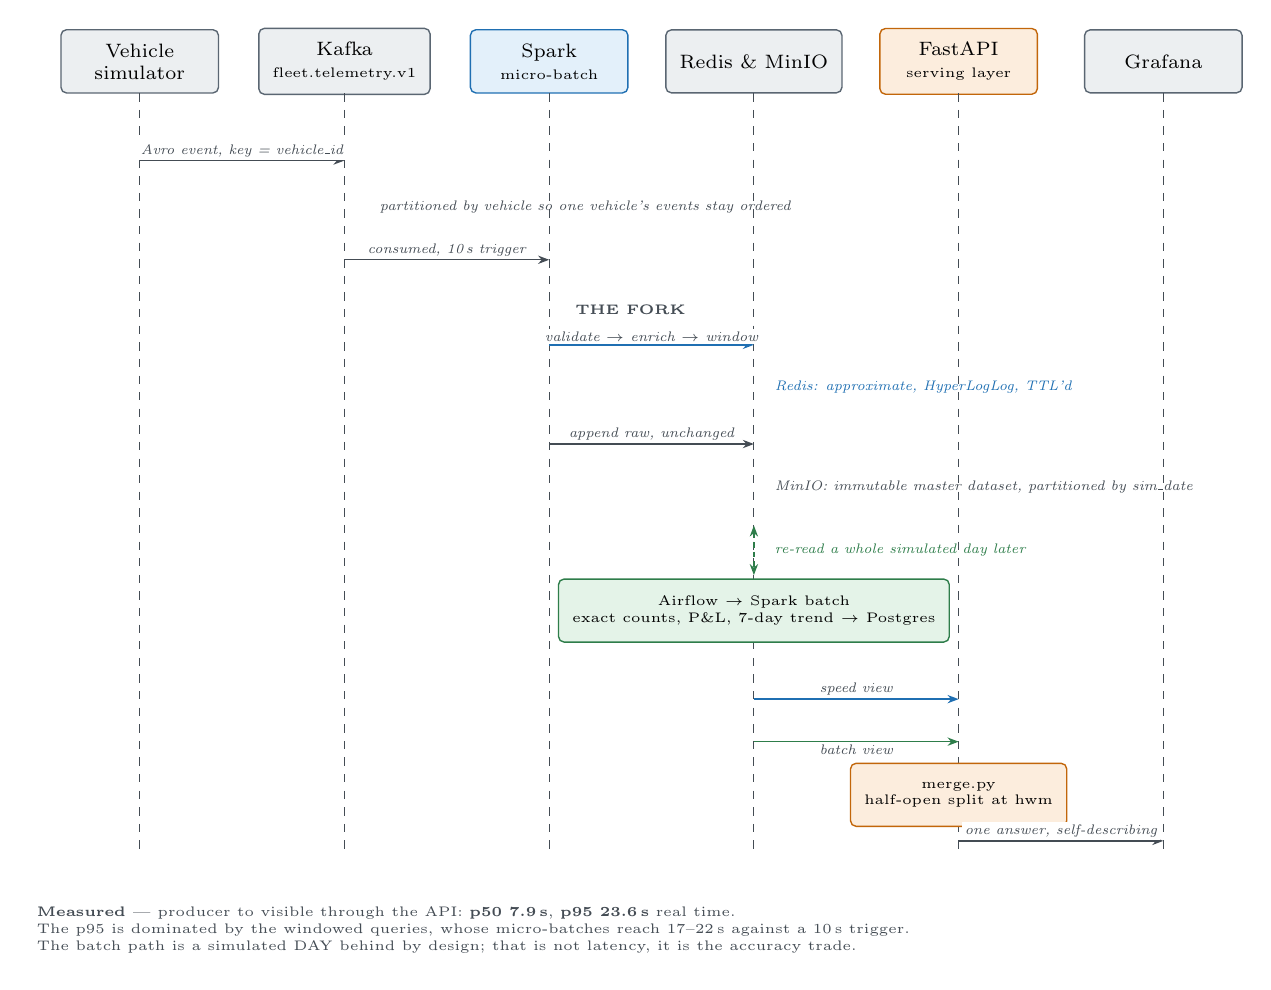
\begin{tikzpicture}[x=26mm, y=9mm]

% ------------------------------------------------------------- lifelines
\foreach \i/\name/\sty in {
    0/{Vehicle\\simulator}/infra,
    1/{Kafka\\\tiny fleet.telemetry.v1}/infra,
    2/{Spark\\\tiny micro-batch}/speed,
    3/{Redis \& MinIO}/infra,
    4/{FastAPI\\\tiny serving layer}/serv,
    5/{Grafana}/infra} {
  \node[\sty, minimum width=20mm, align=center, font=\scriptsize] (h\i) at (\i,1) {\name};
  \draw[edgegrey, dashed, line width=0.3pt] (\i,0.55) -- (\i,-10.2);
}

\newcommand{\msg}[4]{%
  \draw[flow] (#1,#3) -- node[lbl, above, fill=white, inner sep=1pt] {#4} (#2,#3);}

% ------------------------------------------------------------- the stream
\msg{0}{1}{-0.4}{Avro event, key = vehicle\_id}
\node[lbl, anchor=west, text=edgegrey] at (1.15,-1.05)
  {partitioned by vehicle so one vehicle's events stay ordered};

\msg{1}{2}{-1.8}{consumed, 10\,s trigger}

% ---- fork
\node[font=\tiny\bfseries, text=edgegrey, anchor=west] at (2.08,-2.5) {THE FORK};
\draw[speedflow] (2,-3.0) -- node[lbl, above, fill=white, inner sep=1pt]
  {validate $\rightarrow$ enrich $\rightarrow$ window} (3,-3.0);
\node[lbl, anchor=west, text=speedblue] at (3.08,-3.6)
  {Redis: approximate, HyperLogLog, TTL'd};

\draw[flow] (2,-4.4) -- node[lbl, above, fill=white, inner sep=1pt]
  {append raw, unchanged} (3,-4.4);
\node[lbl, anchor=west, text=edgegrey] at (3.08,-5.0)
  {MinIO: immutable master dataset, partitioned by sim\_date};

% ---- batch, a whole simulated day later.
%
% Drawn as a VERTICAL hop down the MinIO lifeline rather than a horizontal message:
% nothing is being sent to another party here, the same data is being re-read later
% by a different process. A horizontal arrow would imply a handoff that never happens.
\draw[batchflow, {Stealth[length=4pt]}-{Stealth[length=4pt]}, dash pattern=on 2pt off 1.5pt]
  (3,-5.55) -- (3,-6.25);
\node[lbl, anchor=west, text=batchgreen] at (3.08,-5.9)
  {re-read a whole simulated day later};
\node[batch, minimum width=32mm, font=\tiny, align=center] at (3,-6.75)
  {Airflow $\rightarrow$ Spark batch\\exact counts, P\&L, 7-day trend $\rightarrow$ Postgres};

% ---- serving
\draw[speedflow] (3,-8.0) -- node[lbl, above, fill=white, inner sep=1pt] {speed view} (4,-8.0);
\draw[batchflow] (3,-8.6) -- node[lbl, below, fill=white, inner sep=1pt] {batch view} (4,-8.6);
\node[serv, minimum width=22mm, font=\tiny, align=center] at (4,-9.35)
  {merge.py\\half-open split at hwm};
\draw[flow] (4,-10.0) -- node[lbl, above, fill=white, inner sep=1pt]
  {one answer, self-describing} (5,-10.0);

% ------------------------------------------------------------- timings
\node[font=\tiny, align=left, anchor=north west, text=edgegrey] at (-0.55,-10.8)
  {\textbf{Measured} \textemdash\ producer to visible through the API:
   \textbf{p50 7.9\,s}, \textbf{p95 23.6\,s} real time.\\
   The p95 is dominated by the windowed queries, whose micro-batches reach 17--22\,s
   against a 10\,s trigger.\\
   The batch path is a simulated DAY behind by design; that is not latency, it is the
   accuracy trade.};

\end{tikzpicture}
\end{document}
